\documentclass[a4paper,pt]{report}

\usepackage[english]{babel}
\usepackage[utf8]{inputenc}
\usepackage{ifthen}
\usepackage{color}
\usepackage{amsmath,amsthm,amssymb,amsfonts}
\usepackage{graphicx}
\usepackage{fancyhdr}

\pagestyle{fancy}


\lhead{\today}
\chead{NSSC II Exercise 4}
\rhead{Group 10}
\cfoot{\thepage}

\begin{document}

\section*{Finite Element Method}
This exercise aims to solve the steady state heat equation using a Finite Element Method.
We consider isotropic elements with $k = 163 \;W/(mK)$ in the first problem statement.
The considered domain is a square of length $L=0.04 m$ with imposed Dirichlet boundary conditions $T=293 \; K$ at the top, homogenous Neumann boundary conditions at the left and right boundary and inhomogenous Neumann boundary conditions $q(y=0)=500000 \; W/m^2$.

\subsection*{Post-Processing}
\subsubsection*{Initial problem}

\begin{figure}
	\centering
	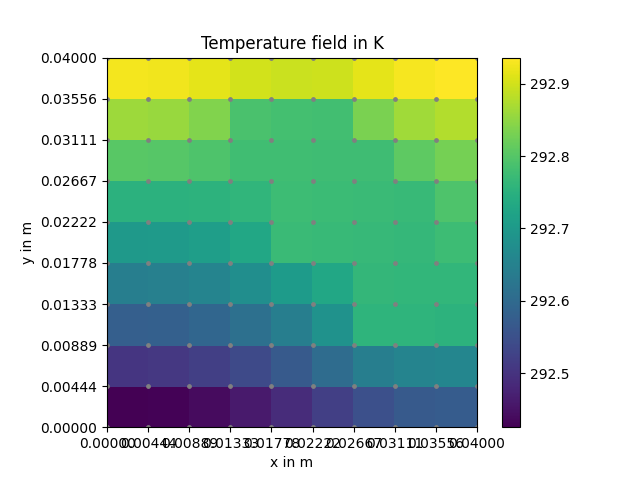
\includegraphics[scale=0.6]{temperaturefield.png}
	\caption{Visualization of the of the solution of the heat equation with the imposed boundary conditions}
	\label{temperaturefield}
\end{figure} 

Figure \ref{temperaturefield} shows the solution of the heat equation and visualizes the temperature at each gridpoint with a linear interpolation between gridpoints. Because of the imposed boundary conditions (heat source at the top, isolation at the left and right boundary) and a material which conducts the heat homogenously inside the domain, we obtain a temperature field $T(x,y)$ which is constant on each vertical line. 
Therefore the partial derivative in x-direction on each triangle is constantly 0 on one hand and the gradient in y-direction is constant as  well. We observe that no heat is being lost at the left and right boundary due to the imposed Neumann boundary conditions. This can be seen in Figure \ref{gradientfield}. 

\begin{figure}
	\centering
	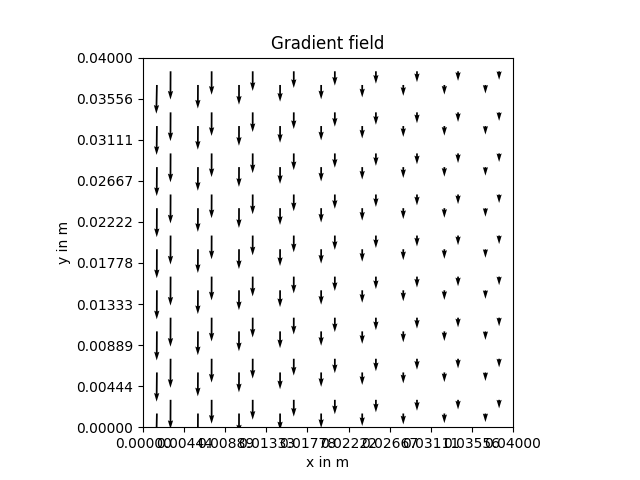
\includegraphics[scale=0.6]{gradientfield.png}
	\caption{Visualization of the gradientfield the of the solution. The local gradients are associated to the centroid of each element}
	\label{gradientfield}
\end{figure}

Since the gradient and the flux are connected by the constitutive law,
\begin{align*}
q_i=-k\frac{\partial }{\partial x_i}T,
\end{align*}
the visualization of the fluxes look similar but with a negative sign, as Figure \ref{fluxes} demonstrates. Summing up all local fluxes, we observe that it is equal to the applied Neumann boundary conditions at the bottom.

\begin{figure}
	\centering
	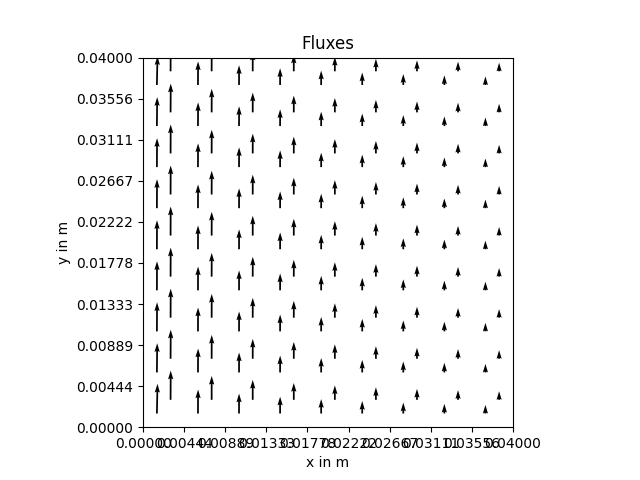
\includegraphics[scale=0.6]{fluxes.png}
	\caption{Visualization of the fluxes.}
	\label{fluxes}
\end{figure}

\subsubsection*{Variation 1}
This variation considers a trapezoidal domain instead of a square. The boundary conditions remain the same. In contrast to the initial problem, we observe that the partial derivative in x direction is not 0 anymore and the gradients are not constant over the whole domain. This yields a different behavior of the temperature in the domain. At the left boundary, the temperature is higher than at the right boundary at a fixed value for the y coordinate. Summing up all local fluxes, we observe that it is equal to the applied Neumann boundary conditions at the bottom anymore.
\begin{figure}
	\centering
	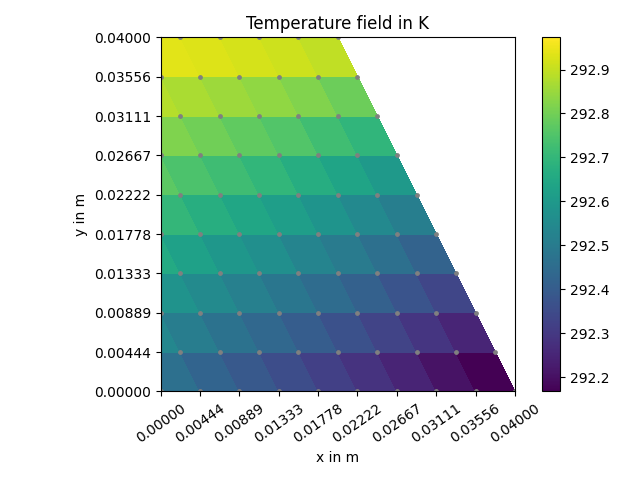
\includegraphics[scale=0.3]{temperaturefieldV1.png}
	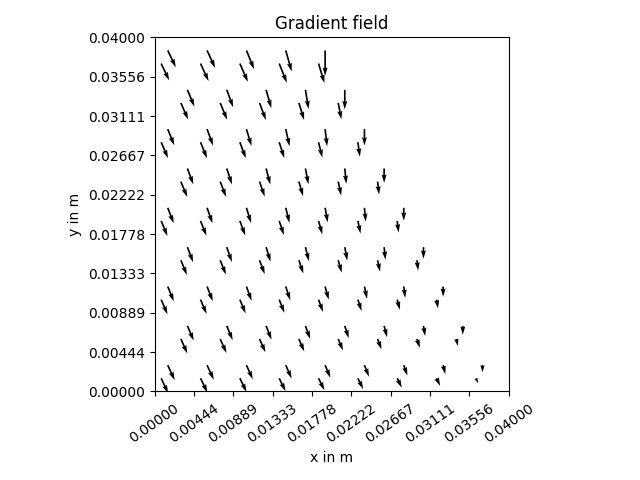
\includegraphics[scale=0.3]{gradientfieldV1.png}
	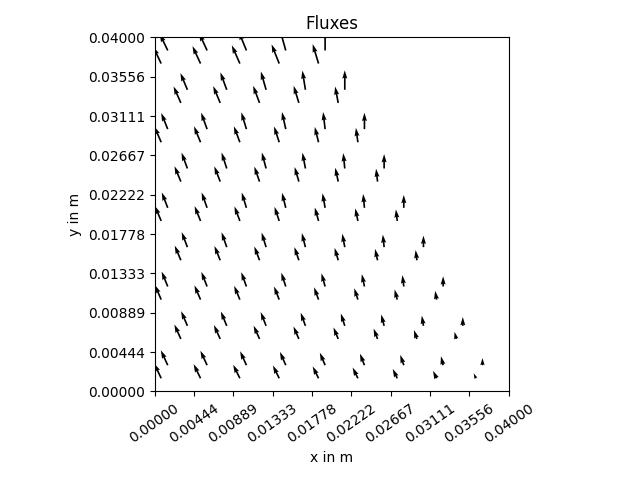
\includegraphics[scale=0.3]{fluxesV1.png}
	\caption{Visualization of the temperature field, the gradient field and the fluxes for variation 1.}
	\label{plotsV1}
\end{figure}

\subsubsection*{Variation 2}
\subsubsection*{Variation 3}
\subsubsection*{Variation 4}

\end{document}